%%%%%%%%%%%%%%%%%%%%%%%%%%%%%%%%%%%%%%%%%%%%%%%%%%%%%%%%%%%%%%%%%%%%%%
% LaTeX: Epistatic control of gene expression
%%%%%%%%%%%%%%%%%%%%%%%%%%%%%%%%%%%%%%%%%%%%%%%%%%%%%%%%%%%%%%%%%%%%%%
%%%%%%%%%%%%%%%%%%%%%%%%%%%%%%%%%%%%%%%%%%%%%%%%%%%%%%%%%%%%%%%%%%%%%%

% Edit the title below to update the display in My Documents
%\title{Epistatic control of gene expression}
%
%%% Preamble
\documentclass[paper=a4, fontsize=11pt]{scrartcl}	% Article class of KOMA-script with 11pt font and a4 format
\usepackage[T1]{fontenc}
\usepackage{fourier}

\usepackage[english]{babel}											% English language/hyphenation
\usepackage[protrusion=true,expansion=true]{microtype}				% Better typography
\usepackage{amsmath,amsfonts,amsthm}								% Math packages
\usepackage[pdftex]{graphicx}										% Enable pdflatex
\usepackage{url}


%%% Custom sectioning (sectsty package)
\usepackage{sectsty}												% Custom sectioning (see below)
\allsectionsfont{\centering \normalfont\scshape}					% Change font of al section commands


%%% Custom headers/footers (fancyhdr package)
\usepackage{fancyhdr}		
\pagestyle{fancyplain}
\fancyhead{}														% No page header
\fancyfoot[L]{}														% Empty 
\fancyfoot[C]{}														% Empty
\fancyfoot[R]{\thepage}												% Pagenumbering
\renewcommand{\headrulewidth}{0pt}									% Remove header underlines
\renewcommand{\footrulewidth}{0pt}									% Remove footer underlines
\setlength{\headheight}{13.6pt}


%%% Equation and float numbering
\numberwithin{equation}{section}									% Equationnumbering: section.eq#
\numberwithin{figure}{section}										% Figurenumbering: section.fig#
\numberwithin{table}{section}										% Tablenumbering: section.tab#


%%% Maketitle metadata
\newcommand{\horrule}[1]{\rule{\linewidth}{#1}} 					% Horizontal rule

\title{
		%\vspace{-1in} 	
		\usefont{OT1}{bch}{b}{n}
		\normalfont \normalsize \textsc{University of Queensland} \\ [25pt]
		\horrule{0.5pt} \\[0.4cm]
		\huge Epistatic control of gene expression in Humans\\[0.3cm]
        \huge *** Report V1 *** \\
		\horrule{2pt} \\[0.5cm]
}
\author{
		\normalfont 								\normalsize
        Joseph Powell\\[-3pt]		\normalsize
        Gibran Hemani\\[0.2cm]		\normalsize
		\today
}
\date{}


%%% Begin document
\begin{document}
\maketitle
\section{Introduction}
In humans expression quantitative trait loci (eQTL) have been extensively studied for their effects on transcript levels as well as their underlying effects on complex phenotypes such as disease susceptibility. To date most studies have analysed SNPs independently and estimated the genotypic effect on mean expression levels assuming an additive mode of inheritance. However, epistasis (gene by gene interactions) is thought to play an important role in the control of gene expression principally through the interaction of transcription factors and the intra-cellular effects of proteins on gene regulation.

The detection of epistasis is significantly hampered by power issues. For example, there is a greater dependency on linkage disequilibrium (LD) between causal variants and observed SNPs in order to capture non-additive variance, and this problem is exacerbated further with epistasis because there must be high LD at all interacting loci. Another obstacle comes from the dependence on a much larger sample size in order to detect similar effect sizes compared to additive effects, because of the increased number of parameters in statistical tests for interaction terms, and the increased multiple testing correction for testing combinations of SNPs. Indeed, most examples of epistasis in humans come from candidate gene studies where multiple testing does not have a detrimental effect. 

Many approaches exist to detect epistasis, many of them are highly parametric, searching for a particular pattern of epistasis or only amongst SNPs with large marginal effects. However, it can be argued that the many patterns of epistasis will go undetected if the search is over-parameterised, and it has been shown that using a test that is agnostic of the epistatic pattern in an exhaustive manner can detect signals that would otherwise go undetected. One method to overcome the problem of excessive multiple testing is to search for interactions in traits, such as gene expression, that are likely to have very large effects, thus improving the power of the study.

Recently we have shown that whilst most genetic variance for gene expression is likely to act in an additive manner, for many probes there exists significant non-additive genetic variance. The importance of epistasis for control of gene expression is largely unknown and has generally not been studied in human populations. It is likely that this is due in part to the considerable computation demands of running a 2D scan on 1000's of probes as well as a restrictive study-wide multiple testing burden. Due to modelling limitations, estimating the genetic variance due to non-additive genetic effects, and epistasis in particular, is often intractable. Thus, searching for epistatic effects directly may serve as a first step in quantifying the contribution of epistasis to complex traits.


%%%%%%%%%%%%%%%%%%%%%%%%
%%%%%%%%%%%%%%%%%%%%%%%%

\section{Methods}

\subsection{Discovery data}

The Brisbane Systems Genetics Study (BSGS) comprises 862 Individuals of European descent from 274 independent families \cite{pmid22563384}. DNA samples from each individual were genotyped on the Illumina 610-Quad Beadchip by the Scientific Services Division at deCODE Genetics Iceland. Full details of genotyping procedures are given in Medland et al. \cite{Medland2009} Standard QC filters were applied and the remaining 528,509 SNPs were carried forward further analysis. 

Gene expression profiles were generated from whole blood collected with PAXgene TM tubes (QIAGEN, Valencia, CA) using Illumina HT12-v4.0 bead arrays. The Illumina HT-12 v4.0 chip contains 47,323 probes, although some probes are not assigned to RefSeq genes. We removed any probes that did not match the following criteria: contained a SNP within the probe sequence with MAF > 0.05 within 1000 genomes data; did not map to a listed ref-seq gene; were not significantly expressed (based on a detection $p$-value < 0.05) in 100\% of samples. After this stringent QC ~7000 [need to get exact number] probes remained for 2d-eqtl mapping. 

\subsection{normalisation}

Gene expression profiles were normalised and batch effects removed with the following procedures; Raw background expression were removed for each sample. Expression levels were then adjusted using Quantile and log2 transformation to standardise distribution between samples. To avoid inflation of the test statistic due to polygenic effects the following linear model was used to correct for batch and polygenic effects;  

\begin{equation}
y = \mu + c + p + s + a + g + e
\label{eq:lm}
\end{equation}
where $\mu$ is the population mean expression levels, $c$, $p$, $s$ and $a$ are vectors of chip, chip position, sex and generation respectively. $g$ is a random additive polygenic effect with a variance covariance matrix 


\begin{equation}
G_{ijk} = \left \{ 
\begin{array}{ll}
\sigma _a ^2 + \sigma _e ^2&        j = k \\ 
2\phi _{ijk} \sigma _a ^2& 			j \neq k \\
\end{array} \right.
\end{equation}

The parameters $\sigma _a ^a$ and $\sigma _e ^2$ are variance components for additive background genetic and environmental effects respectively. Here, we are using family based pedigree information rather than SNP based IDB to account for relationships between individuals and so $\phi _{ijk}$ is the kinship coefficient between individuals $j$ and $k$. The residual, $e$, from equation \ref{eq:lm} are assumed to follow a multivariate normal distribution with a mean of zero. These residuals are corrected for batch, sex, generation and polygenic effects. Residuals were standardised to Z-scores using a inverse-normal transformation and used as the adjusted phenotype for the pairwise epistasis scan. 

\subsection{exhaustive 2d-eQTL analysis}
We used epi-GPU software to perform an exhaustive scan for pairwise interactions, such that each SNP is tested against all other SNPs for statistical association with the expression values for each of the ~7000 probes. For each SNP-pair there are 9 possible genotype classes. We treat each genotype class as a fixed effect and fit an 8 d.f. $F$-test to test the following hypotheses:

\begin{equation}
H _0 : \sum _{i=1} ^3 \sum _{j=1} ^3 (\bar x _{ij} - \mu) ^2 = 0; 
\end{equation}

\begin{equation}
H _1 : \sum _{i=1} ^3 \sum _{j=1} ^3 (\bar x _{ij} - \mu) ^2 > 0; 
\label{eq:8df}
\end{equation}

where $\mu$ is the mean expression level and $x _{ij}$ is the pairwise genotype class mean for genotype $i$ at SNP 1 and genotype $j$ at locus B. This type of test does not parameterize for specific types of epistasis, rather it tests for the joint genetic effects at two loci. This has been demonstrated to be statistically more efficient when searching for a wide range of epistatic patterns (add refs), although will include any marginal effects of SNPs. \\[0.2cm]
 
The complete exhaustive scan for 7,000 probes comprises of $\sim$9.8$e^{14}$ $F$-tests. Due to the very large number of tests [plus nature of epistasis ....] we used a highly conservative series of filtering steps to identify study-wide significant epistasis associations to follow forward for replication analysis. Initially a significance threshold of $-log10$ 15.5. This threshold is the study-wide significance threshold determined by the number of independent tests for a 2D scan for a single probe / the number of probes analysed. This is likely to be conservative as this threshold assumes independence between probes. Following filtering on this threshold only SNP pairs with all 9 genotype classes and minimum genotype class size > 5 individuals were kept. We then calculated the linkage disequilibrium between SNPs in a pair and removed any pairs with $r^2$ > 0.1. We also removed any pairs containing SNPs for which single marker additive or dominance effects had been identified  in previous work (Powell et al. in Press). Sentinel  SNP pairs we retained from epistasis eQTL 'peaks' comprising of multiple sets of pair-wise SNPs. At this stage $\sim$13,000 SNP pairs remained and were tested for the contribution of marginal and interaction terms by testing the 8d.f. \ref{eq:8df} verses a 4 d.f. model parameterizing for interaction terms only:

\begin{equation}
H _0: \sum _{i=1} ^3 \sum _{j=1} ^3 (\bar x _{ij} - \bar x _i - \bar x _j + \mu) ^2 = 0;
\end{equation}

\begin{equation}
H _1: \sum _{i=1} ^3 \sum _{j=1} ^3 (\bar x _{ij} - \bar x _i - \bar x _j + \mu) ^2 > 0;
\label{eq:4df}
\end{equation}

where $\bar x _i (\bar x _j)$ is the marginal class mean for genotype $i (j)$ at SNP A (B). Significance of interaction terms was determined using a bonferroni threshold of $0.05 / 13000 = 3.8e^{-6}$ 


\subsubsection{Fine mapping}

To assess the impact of pair-wise epistasis variants not present on the Illumina 610Q beadchip and better define the association regions, we imputed genotypes in the region 100kb upstream and downstream of the sentinel SNPs using the full reference panel from the 1000 Genomes Project. The quality of imputation was assessed by means of the $R^2$ statistic. Used a highly conservative threshold, we removed any SNPs with $R^2 < 0.9$. Thus, or each epistasis pair two imputed SNP blocks were carried forward for fine mapping analysis. Each pairwise combination of SNPs in blocks 1 and 2 were tested in a ful 8d.f. and reduced (interaction) 4d.f. model. As before any SNP pairs not matching the criteria of $r^2$  < 0.1, number of genotype classes = 9, and minimum genotype class size > 5 were removed from the output. 

This approach allows us to fine map to the causal epistatic loci. Given the nature epistasis genetic variance, any snp pairs with large estimate of non-additive genetic variance are very unlikely to be rare. Therefore, fine mapped loci provide good functional candidates. Hereon, results from the original 2D scan using genotyped SNPs will be refered to as genotype pairs and results from the fine mapping 2D scan using imputed data will be termed imputed pairs. Thus, for each significant pair there will be a results from genotyped and imputed pairs. However, as fine mapping includes a large number of additional tests, any oberved increases in the interaction (4d.f.) $p$-values could be due to chance arising from multiple testing. To address this we ran a series of simulations to determine the empirical change from genotype interaction $p$-value to imputed interaction $p$-value expected in situations where no epistatic exists. For the following three scenarios; $cis-cis$, $cis-trans$ and $trans-trans$ we randomly selected a probe for which no significant epistatic genotype pairs had been identified and randomly selected two SNP blocks within the defined genomic regions. The SNP pair was tested using the 4 and 8d.f. models and then imputed SNPs were extracted from 100kb upstream and downstream regions. Pairwise interactions were tested for the SNPs in the two imputed blocks and the SNP pair with the minimum interaction $p$-value retained. This process was repeated 10,000 times for each of the three scenarios.   

     


\subsection{replication}  

We have attempted replication of the 2D scan significant results using three independent cohorts; Fehrmann, CHDWB and Rotterdam. Details of cohorts are as follows. \\[0.1cm]  

Fehrmann: $n$=1,469 \\[0.1cm]
The Fehrmann dataset consists of whole peripheral blood samples of 1,469 unrelated individuals from the United Kingdom and the Netherlands. Some of these individuals are patients, while others are healthy controls. Individuals were genotyped using Illumina HumanHap300, HumanHap370 or the 610 Quad platform. RNA levels were quantified using both the Illumina H8v2 platform (N = 229) and the HT12v3 platform (N = 1,240). \\[0.1cm]

CDHWB: $n$=189 \\ [0.1cm]
The Center for Health Discovery and Well Being (CDHWB) Study is a population based cohort consisting of 189 individuals collected in Atlanta USA. Gene expression profiles were generated with Illumina HT-12 V3.0 arrays from whole blood collected from Tempus tubes that preserve RNA. Whole genome genotypes were measured using Illumina OmniQuad arrays. \\[0.1cm]

Rotterdam: $n$=762 \\[0.1cm]
The Rotterdam Study is a large population based cohort collected to investigate the prevalence, incidence, and risk factors of chronic diseases among  Caucasians aged 45 years and over. Participants were genotyped using the Illumina 610K quad arrays. Whole blood of 768 samples was collected (PAXgene)and RNA hybridized to the Illumina Human HT-12v4 chips.

\subsection{Functional characterisation}

[From Kostya]

\section{Results}

\subsection{2D Scan}

We performed exhaustive two-dimensional searches on 7339 expression probes, identifying 432 significant pairwise interactions on 218 probes. We decomposed the genotype-phenotype map into parametric variance components and observed that there was no enrichment for any particular epistatic variance component amongst the significant SNPs (Table \ref{tab:vc}), demonstrating that a search that is agnostic of the pattern of epistasis is likely to detect things that would otherwise be missed. The majority of significant interactions were found to have a `cis-trans' effect (Table \ref{tab:type}; \emph{i.e.} one SNP was on the same chromosome as the probe while the other was on a different chromosome). Of the 218 probes, 78 had more than one significant interaction (Figure \ref{fig:circos})


\begin{table}[ht]
	\centering
	\begin{tabular}{rlr}
		\hline
		& Interaction type & Freq \\ 
		\hline
		1 & $cis-cis$ &  32 \\ 
		2 & $cis-trans$ & 388 \\ 
		3 & $trans-trans$ &  12 \\ 
		\hline
	\end{tabular}
	\caption{Epistasis pair positions. Here $cis$ SNPs are on the same chromosome as the probe. $Trans$ SNPs are on a different chromosome}
	\label{tab:type}
\end{table}

\begin{table}[ht]
	\centering
	\begin{tabular}{rlr}
		\hline
		& Main epistatic effect & Freq \\ 
		\hline
		1 & A x A &  99 \\ 
		2 & A x D &  93 \\ 
		3 & D x A & 117 \\ 
		4 & D x D & 123 \\ 
		\hline
	\end{tabular}
	\caption{The largest epistatic variance component was recorded for each pair. This table summerises how often each type of epistatic variance occurs}
	\label{tab:vc}
\end{table}

\begin{figure}[p]
	\centering
	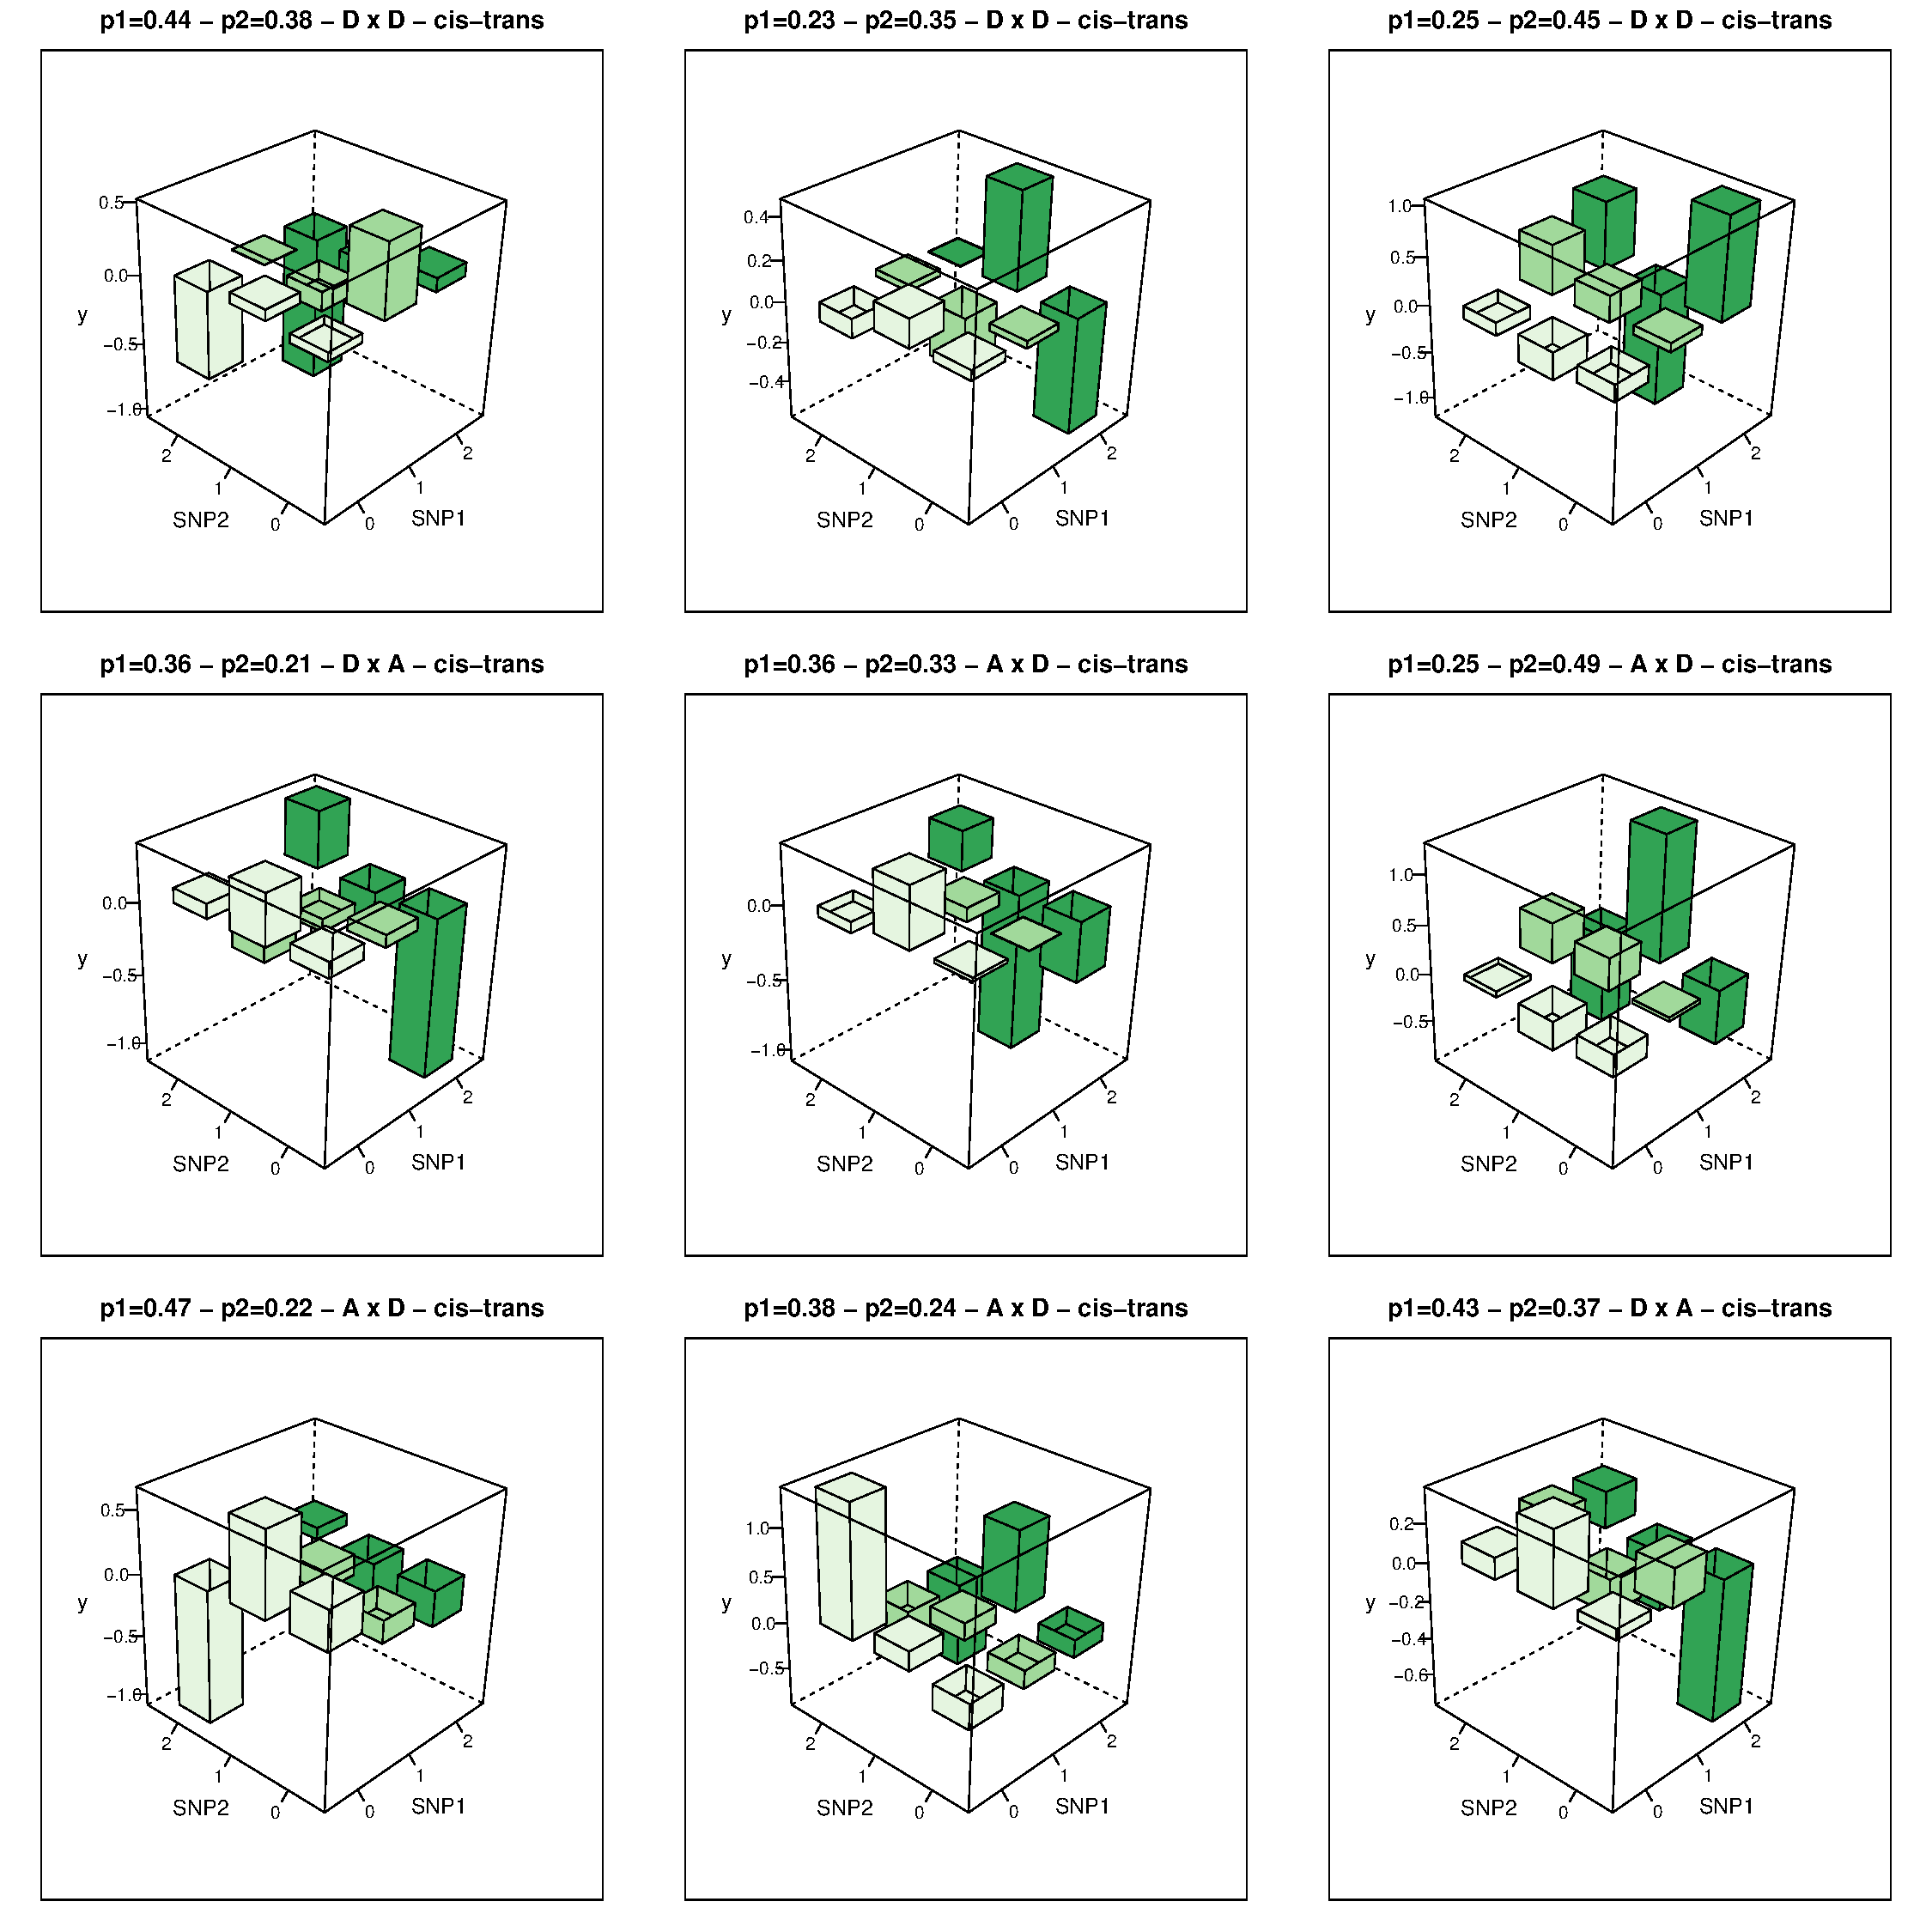
\includegraphics[width=15cm]{images/3dplots}
	\caption{Genotype-phenotype maps for the nine most significant interactions. p1 and p2 are MAF for SNP 1 and SNP 2 respectively}
	\label{fig:3dplots}
\end{figure}

\begin{figure}[p]
	\centering
	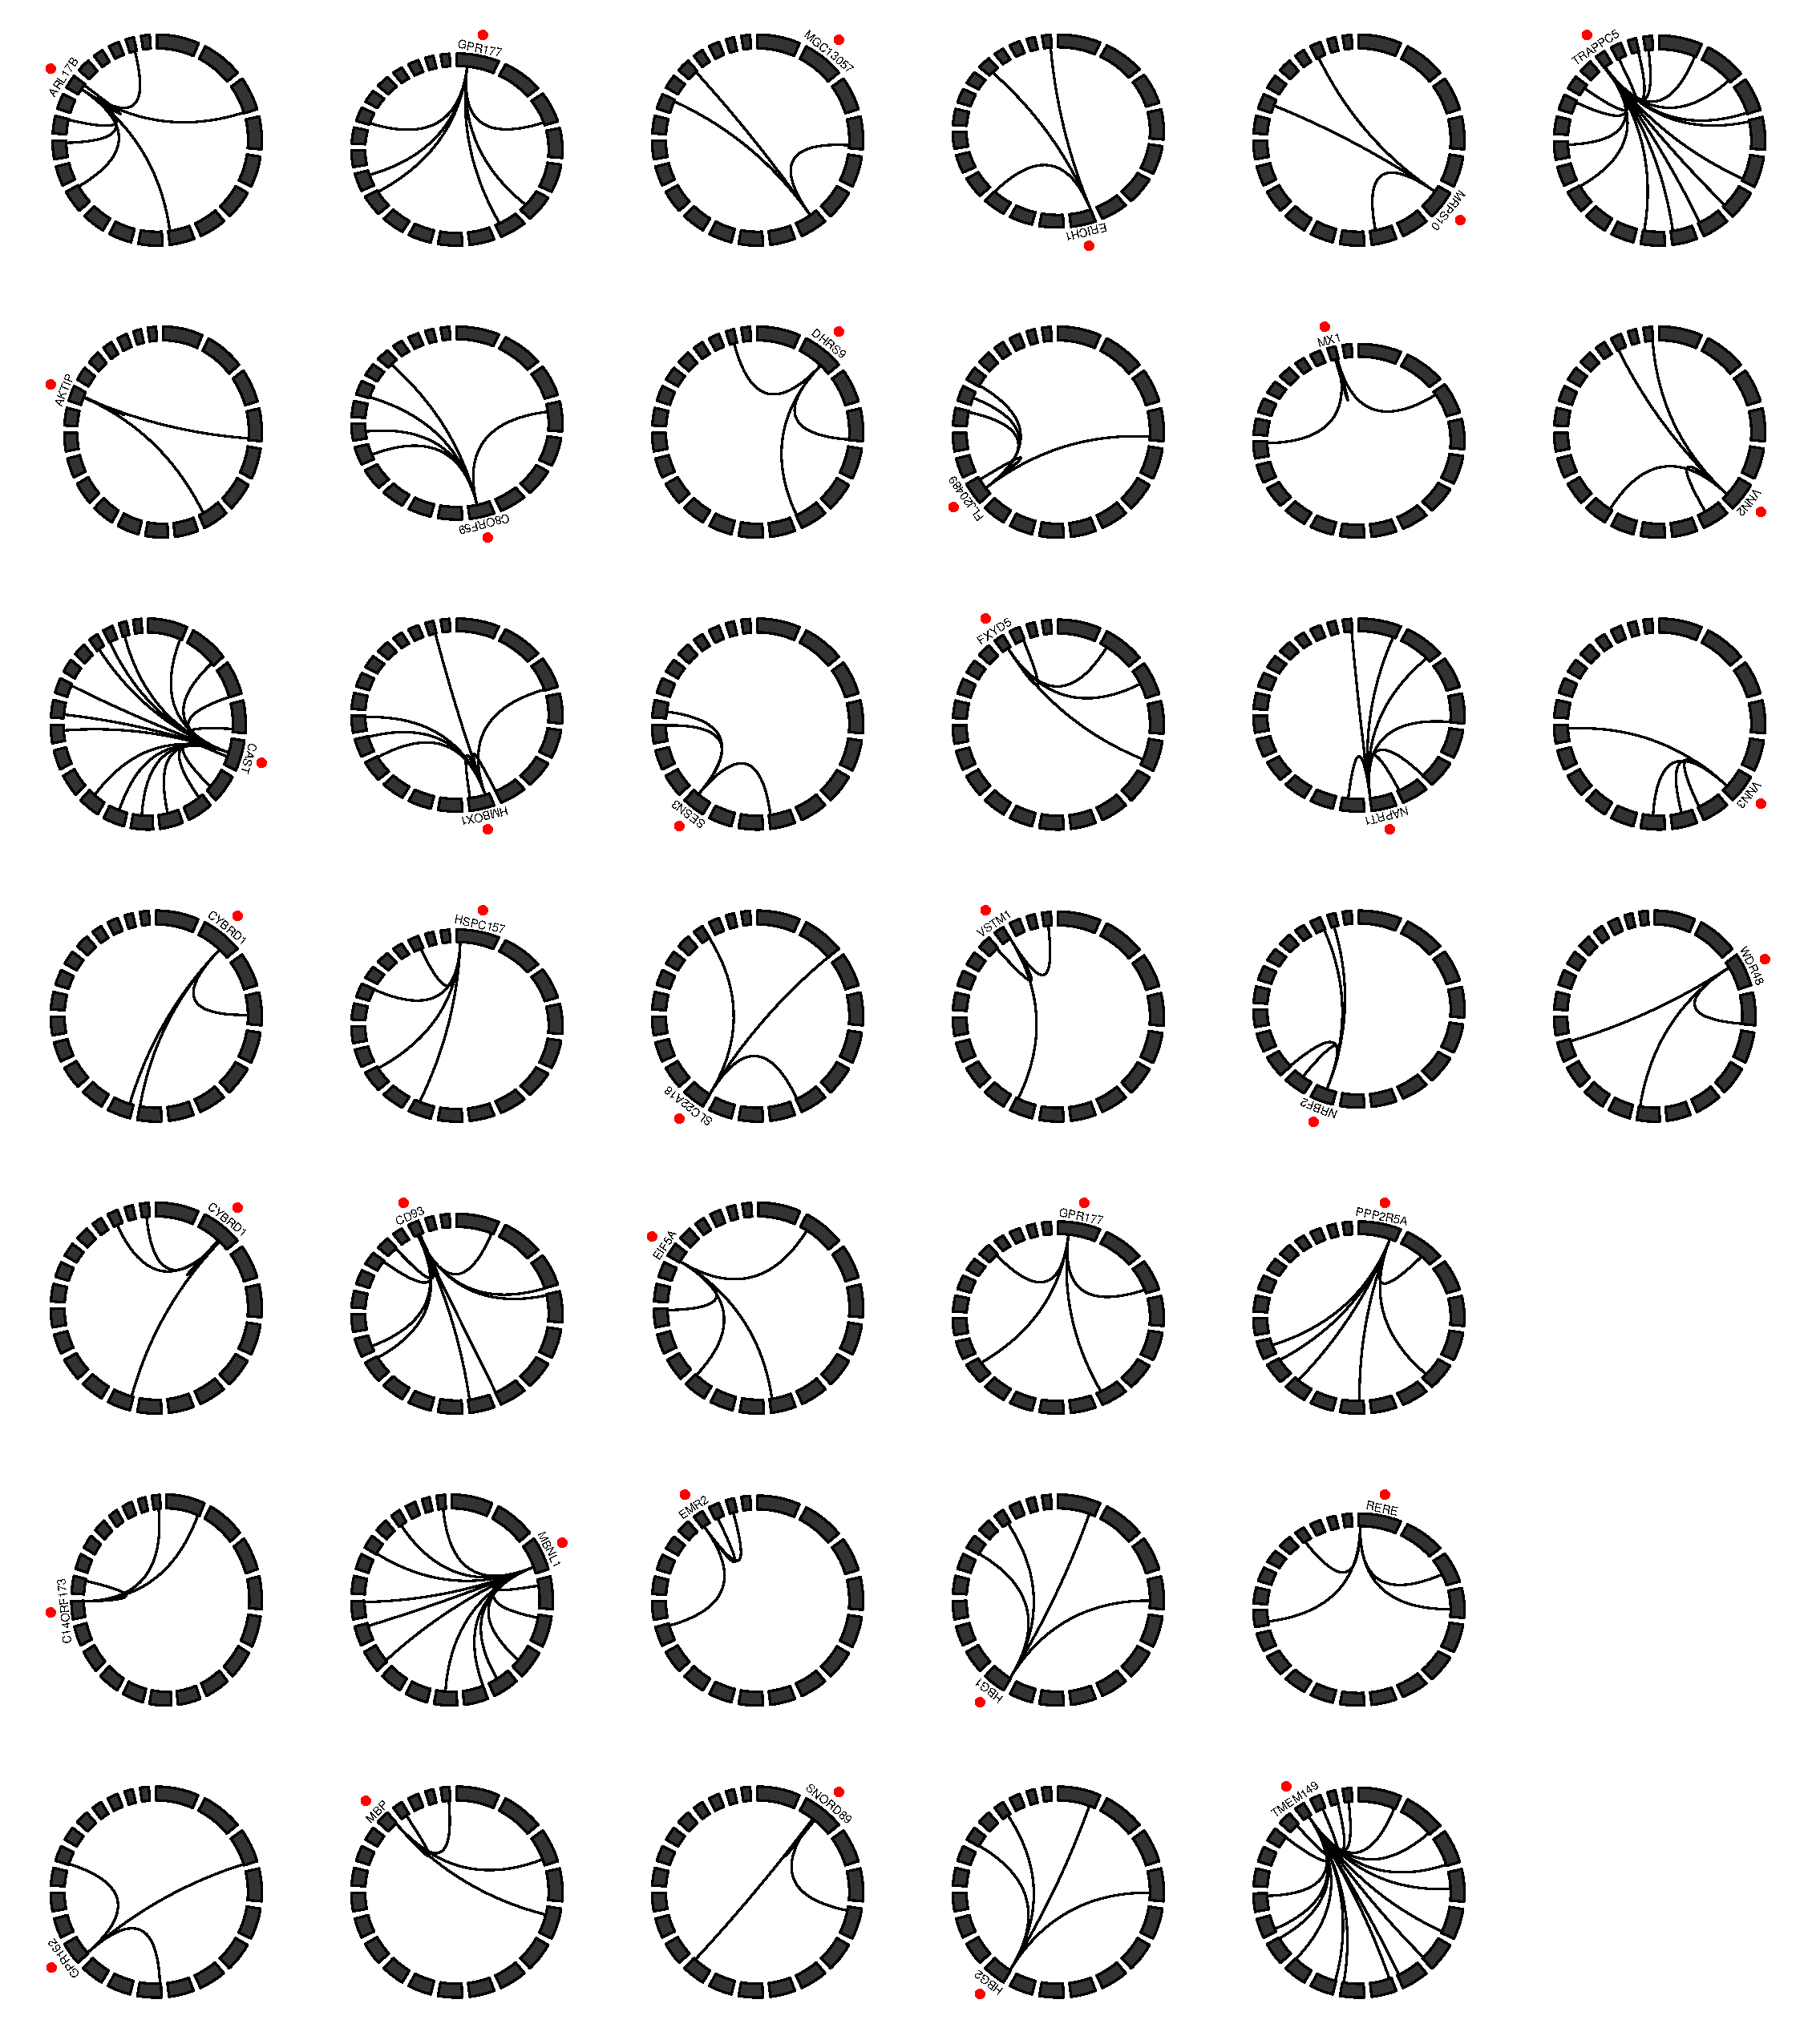
\includegraphics[width=15cm]{images/circos}
	\caption{Genomic maps for 39 probes that have two or more significant interactions. The red dot denotes the chromosome where the probe resides and arcs denote interacting SNP pairs.}
	\label{fig:circos}
\end{figure}



\subsection{Additive vs non-additive}

This study has focused on identifying statistical interactions, however all significant interactions exhibit relatively large additive genetic effects (Figure \ref{fig:proportion_additive}).

\begin{figure}[p]
	\centering
	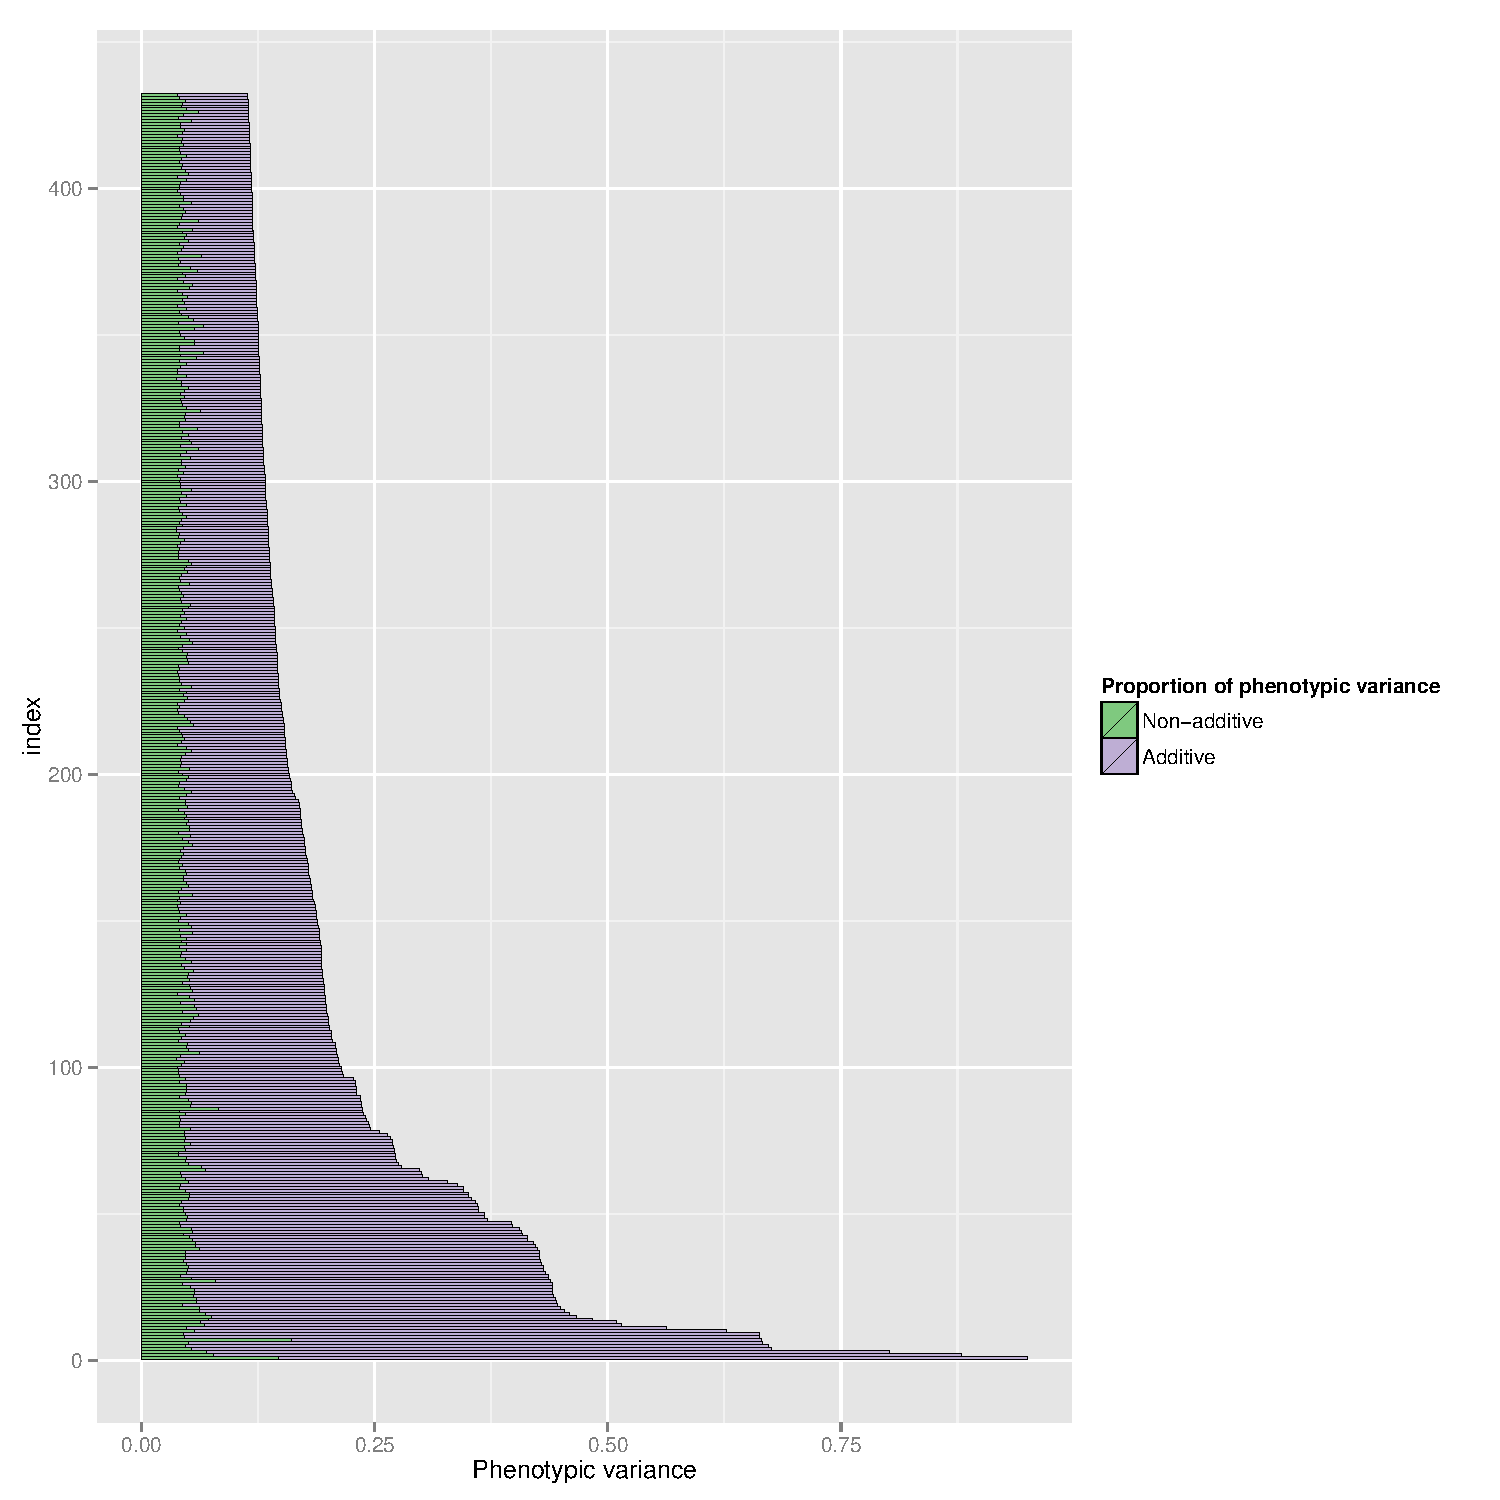
\includegraphics[width=15cm]{images/proportion_additive}
	\caption{Proportion of genetic variance attributed to additive and non-additive effects, ranked in order of total genetic variance explained by the interacting SNP pair.}
	\label{fig:proportion_additive}
\end{figure}



\subsection{Replication}


We attempted replication of the signals in an independent dataset [Greg Gibson - 139 individuals, 185 out of 432 interactions had both SNPs in common in the two datasets]. We observed no significant $p$-values after adjusting for multiple testing (lowest $p$-value$=0.0099$ in replication dataset, threshold set at $0.05/185=0.0003$). We tested for enrichment of $p$-values but there was no evidence of departure from the null hypothesis of no effects (Figure \ref{fig:gg_replication}). 

Replication in Fehrmann and EGCUT

Of the 432 probe by SNP pair associations supplied to the replication group(s) 387 and 391 were present at the desired criteria in Fehrmenn and EGCUT respectively.

\begin{table}[ht]
	\centering
	\begin{tabular}{rrrr}
	\hline
	& & Fehrmann & EGCUT \\
	\hline
	P value & Expected & Observed & Observed \\
	\hline	  
	0.1 & 38 & 51 & 67 \\
	0.05 & 19 & 35 & 44 \\
	0.01 & 4 & 22 & 26 \\
	0.001 & <1 & 14 & 22 \\
	0.0001 & ~0 & 7 & 17 \\
	\hline
	\end{tabular}
\end{table}


\begin{table}[ht]
\centering
\begin{tabular}{rrrrrllrlrrrrr}
  \hline
chr1 & chr2 & pos1 & pos2 & snp1 & snp2 & probechr & probegene & snpcor & replication\_pnest & replication\_r & replication\_nclass & replication\_minclass \\ 
  \hline
19 &  19 & 483171 & 483155 & rs807491 & rs7254601 &  19 & TMEM149 & 0.02 & 81.55 & 0.05 &   9 &  16 \\ 
19 &  19 & 481151 & 481145 & rs873870 & rs7252981 &  19 & ATP13A1 & -0.26 & 48.72 & -0.34 &   9 &  12 \\ 
11 &  11 & 345268 & 345257 & rs7930237 & rs556895 &  11 & CTSC & -0.11 & 18.76 & 0.09 &   9 &   8 \\ 
10 &  10 & 317649 & 317615 & rs2395095 & rs10824092 &  10 & ADK & 0.12 & 18.33 & 0.10 &   9 &  13 \\ 
8 &   8 & 277063 & 277044 & rs2123758 & rs3889129 &   8 & NAPRT1 & 0.23 & 15.12 & 0.18 &   9 &  34 \\ 
3 &   3 & 110710 & 110699 & rs16864367 & rs13069559 &   3 & MBNL1 & 0.29 & 10.30 & 0.23 &   9 &   9 \\ 
14 &   3 & 416822 & 110699 & rs2614467 & rs13069559 &   3 & MBNL1 & -0.02 & 4.13 & 0.03 &   9 &  12 \\ 
19 &   8 & 483165 & 252775 & rs8106959 & rs1843357 &  19 & TMEM149 & 0.02 & 3.72 & -0.00 &   9 &  10 \\ 
19 &   3 & 483165 & 117001 & rs8106959 & rs10937361 &  19 & TMEM149 & 0.01 & 3.61 & -0.00 &   9 &  12 \\ 
8 &   3 & 257325 & 117283 & rs8180944 & rs4553956 &   8 & HMBOX1 & 0.05 & 3.38 & -0.05 &   9 &   4 \\ 
19 &   1 & 483165 & 38950 & rs8106959 & rs914940 &  19 & TMEM149 & 0.04 & 3.36 & -0.05 &   9 &   8 \\ 
19 &   2 & 483165 & 80806 & rs8106959 & rs6718480 &  19 & TMEM149 & 0.02 & 3.31 & -0.02 &   9 &  10 \\ 
19 &   6 & 483165 & 216524 & rs8106959 & rs6926382 &  19 & TMEM149 & -0.05 & 3.06 & -0.03 &   9 &  12 \\ 
19 &  14 & 483165 & 414535 & rs8106959 & rs17719594 &  19 & TMEM149 & 0.04 & 3.06 & 0.02 &   9 &  12 \\ 
5 &   3 & 155373 & 110699 & rs7710738 & rs13069559 &   3 & MBNL1 & 0.10 & 2.55 & -0.03 &   9 &   9 \\ 
19 &  12 & 483165 & 379273 & rs8106959 & rs1401098 &  19 & TMEM149 & -0.01 & 2.41 & 0.04 &   9 &  11 \\ 
17 &  15 & 450341 & 430903 & rs1533031 & rs12591171 &  17 & XAF1 & -0.04 & 2.38 & -0.03 &   9 &   9 \\ 
14 &   8 & 406922 & 265704 & rs7152284 & rs2896452 &   8 & C8ORF59 & 0.02 & 2.18 & 0.07 &   9 &  17 \\ 
19 &   5 & 483884 & 178750 & rs4803481 & rs2421050 &  19 & CEACAM21 & 0.07 & 2.16 & -0.02 &   9 &   9 \\ 
7 &   1 & 242078 & 11854 & rs12532999 & rs12065581 &   1 & GPR177 & -0.08 & 2.13 & 0.04 &   9 &  10 \\ 
   \hline
\end{tabular}
\end{table}


\begin{table}[ht]
\centering
\begin{tabular}{rrrrrllrlrrrrr}
  \hline
chr1 & chr2 & pos1 & pos2 & snp1 & snp2 & probechr & probegene & snpcor & replication\_pnest & replication\_r & replication\_nclass & replication\_minclass \\ 
  \hline
19 &  19 & 483171 & 483155 & rs807491 & rs7254601 &  19 & TMEM149 & 0.02 & 45.78 & -0.13 &   9 &   3 \\ 
19 &  19 & 481151 & 481145 & rs873870 & rs7252981 &  19 & ATP13A1 & -0.26 & 42.37 & 0.37 &   9 &   3 \\ 
10 &  10 & 317649 & 317615 & rs2395095 & rs10824092 &  10 & ADK & 0.12 & 21.21 & -0.04 &   9 &  11 \\ 
3 &   3 & 110710 & 110699 & rs16864367 & rs13069559 &   3 & MBNL1 & 0.29 & 20.36 & 0.18 &   9 &   4 \\ 
8 &   8 & 277063 & 277044 & rs2123758 & rs3889129 &   8 & NAPRT1 & 0.23 & 16.08 & 0.01 &   9 &  29 \\ 
11 &  11 & 345268 & 345257 & rs7930237 & rs556895 &  11 & CTSC & -0.11 & 15.06 & 0.19 &   9 &   2 \\ 
19 &   4 & 483165 & 137487 & rs8106959 & rs2351458 &  19 & TMEM149 & 0.03 & 9.61 & -0.02 &   9 &   4 \\ 
19 &   6 & 483165 & 216524 & rs8106959 & rs6926382 &  19 & TMEM149 & -0.05 & 8.80 & -0.03 &   9 &   6 \\ 
5 &   3 & 155373 & 110699 & rs7710738 & rs13069559 &   3 & MBNL1 & 0.10 & 7.89 & 0.05 &   9 &   4 \\ 
19 &   1 & 483165 & 38950 & rs8106959 & rs914940 &  19 & TMEM149 & 0.04 & 6.96 & 0.01 &   9 &   3 \\ 
17 &   3 & 450326 & 110699 & rs218671 & rs13069559 &   3 & MBNL1 & -0.03 & 5.82 & 0.00 &   9 &   4 \\ 
6 &   3 & 207083 & 110699 & rs2030926 & rs13069559 &   3 & MBNL1 & 0.05 & 5.80 & -0.00 &   9 &   1 \\ 
19 &  13 & 483165 & 380931 & rs8106959 & rs9509428 &  19 & TMEM149 & -0.01 & 5.75 & -0.01 &   9 &   2 \\ 
7 &   3 & 236869 & 110699 & rs11981513 & rs13069559 &   3 & MBNL1 & 0.02 & 5.36 & 0.00 &   9 &   5 \\ 
19 &   2 & 483165 & 80806 & rs8106959 & rs6718480 &  19 & TMEM149 & 0.02 & 5.15 & -0.07 &   9 &   1 \\ 
4 &   3 & 126893 & 110699 & rs4392535 & rs13069559 &   3 & MBNL1 & 0.02 & 4.33 & -0.02 &   9 &   1 \\ 
8 &   3 & 248082 & 110699 & rs4735830 & rs13069559 &   3 & MBNL1 & 0.03 & 4.21 & -0.05 &   9 &   4 \\ 
19 &  11 & 483165 & 353621 & rs8106959 & rs471728 &  19 & TMEM149 & 0.04 & 3.62 & 0.04 &   9 &   4 \\ 
19 &   8 & 483165 & 252775 & rs8106959 & rs1843357 &  19 & TMEM149 & 0.02 & 3.33 & -0.04 &   9 &   2 \\ 
19 &  17 & 483165 & 462278 & rs8106959 & rs7213338 &  19 & TMEM149 & 0.04 & 3.14 & 0.04 &   9 &   7 \\ 
   \hline
\end{tabular}
\end{table}


\begin{figure}[p]
	\centering
	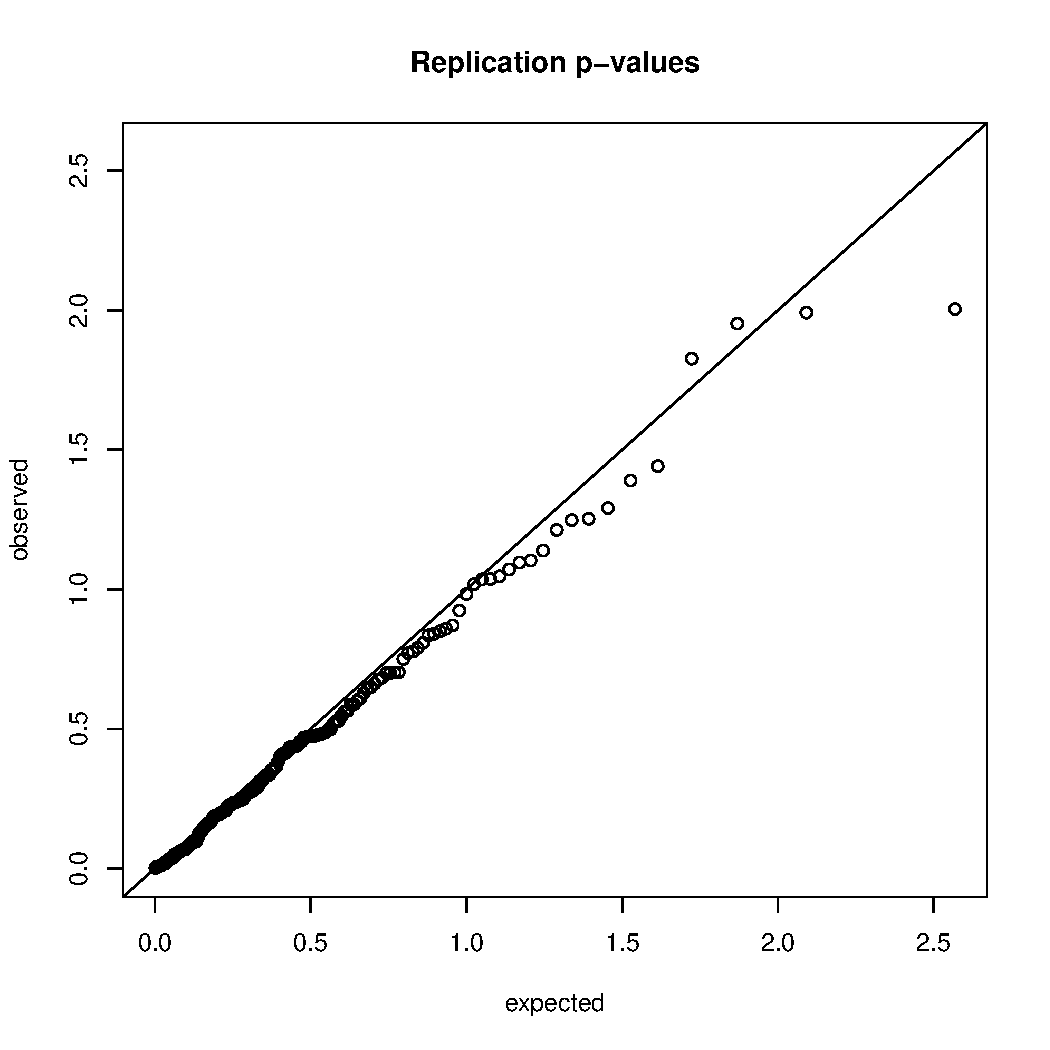
\includegraphics[width=15cm]{images/replication_qqplot}
	\caption{Q-Q plot for interaction $p$-values (4 degrees of freedom) for 185 interactions that had SNPs in common in the replication dataset.}
	\label{fig:gg_replication}
\end{figure}



\begin{figure}[p]
	\centering
	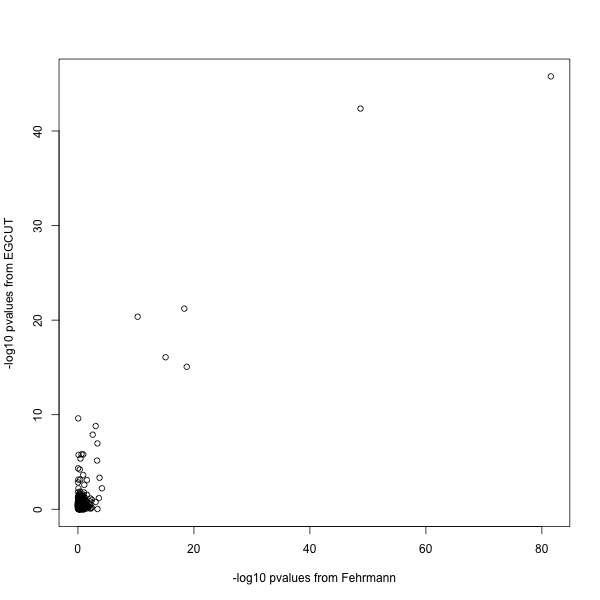
\includegraphics[width=15cm]{images/EGCUT_vs_Fehrmann_all}
	\caption{-log10 pvalues for all snp / probe pairs in Fehrnmann and EGCUT}
	\label{fig:repl_match}
\end{figure}

\begin{figure}[p]
	\centering
	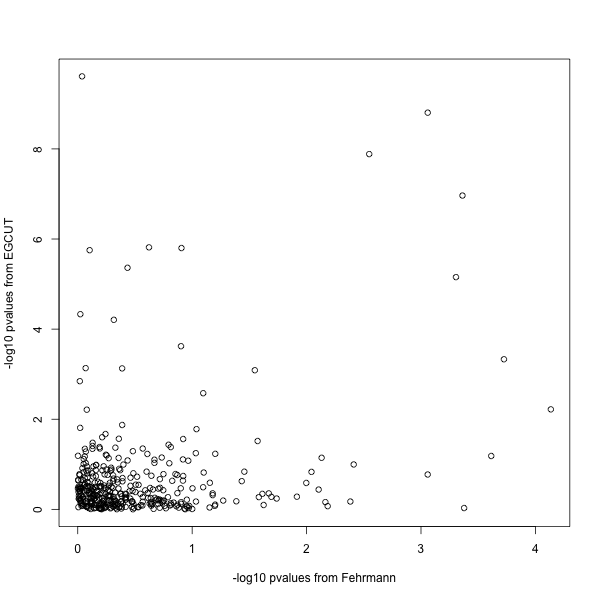
\includegraphics[width=15cm]{images/EGCUT_vs_Fehrmann_pval10}
	\caption{-log10 pvalues for all snp / probe pairs with -log10 p values less than 10 in Fehrnmann and EGCUT datasets}
	\label{fig:repl_match10}
\end{figure}




\subsection{Fine Mapping}

\subsection{Functional characterisation}


%%% Refs
\clearpage
\bibliographystyle{plain}
\bibliography{report_v1_refs}


%%% End document
\end{document}